\noindent\textbf{About this recipe:}\\
This recipe will make you delicious, buttery fluffy brioche buns. They
can be eaten on its own or used as a basis for burgers. This is my goto recipe
that I have perfected over the years. They can be made both with sourdough and
yeast. The yeasted buns are typically ready within 1 to 2 hours whereas the
sourdough buns will take around 10~hours to complete.

They can also be frozen and stored for an extended period of time. This
way you will always have fresh buns at hand.

To really make them shine it is essential to include a high buttery content.
This makes them softer and improves the taste. Furthermore no water is used,
the milk will improve the softness even further.

\begin{figure}[h]
    \centering
    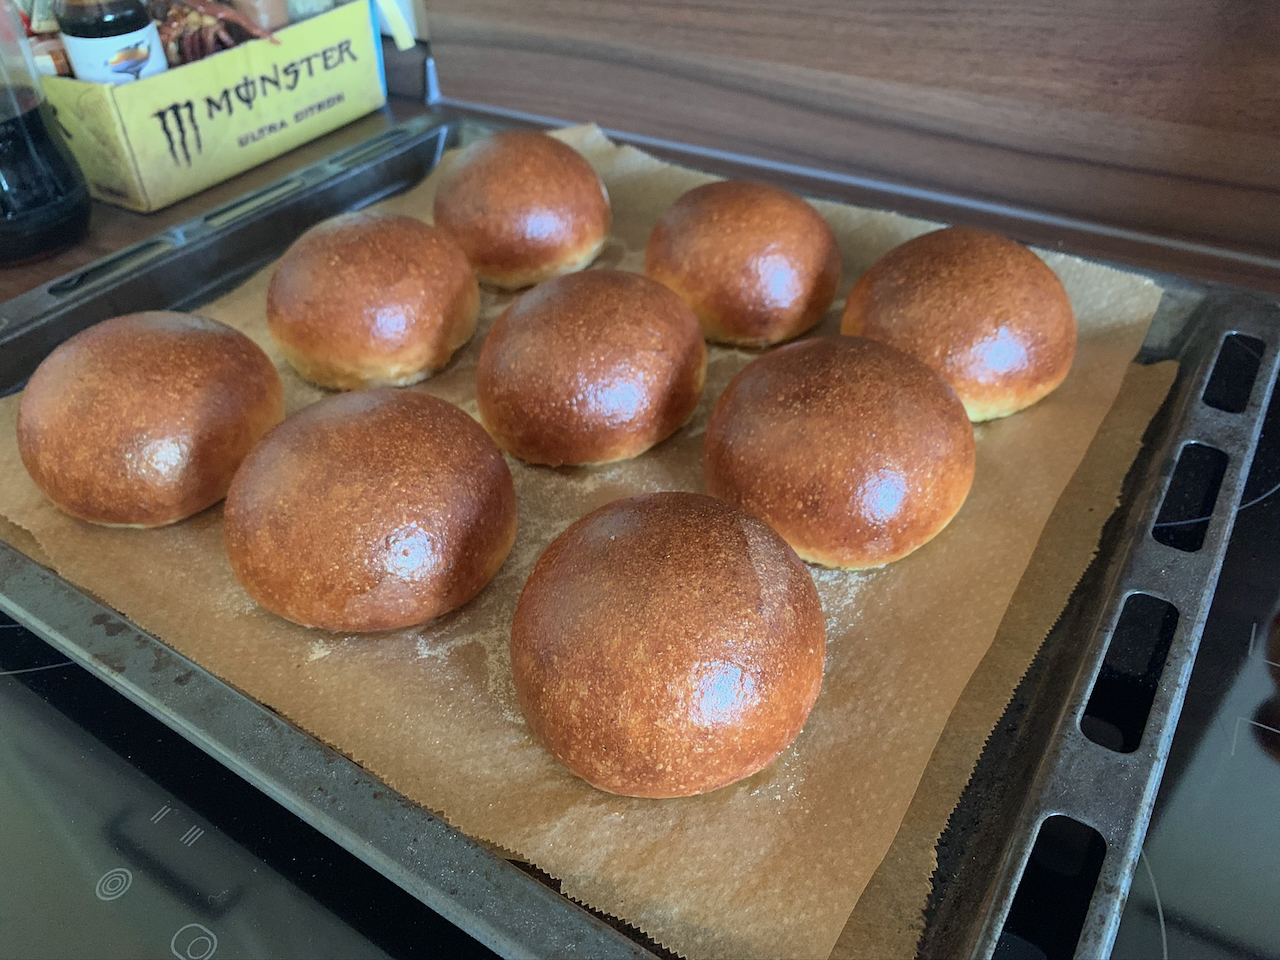
\includegraphics[width=\textwidth]{brioche-buns}
    \caption{Fluffy buttery brioche buns. The perfect burger companion.}
\end{figure}

\noindent\textbf{Ingredients:}

\begin{center}
\begin{tabular}{|c|l|r|r|}
    \hline
    \textbf{No.} & \textbf{Ingredient} & \textbf{Quantity} & \textbf{Baker's math} \\
    \hline
    1 & All purpose flour & 500 g = 8 buns & 100\% \\
    \hline
    2 & Milk, warm & 200 g & 40\% \\
    \hline
    4 & Butter, warm & 200 g & 40\% \\
    \hline
    3 & Eggs & 2pc & 1 per 250 g flour \\
    \hline
    4 & Sugar & 50 g & 10\% \\
    \hline
    5 & Salt & 10 g & 2\% \\
    \hline
    6 & Sourdough starter & 50 g & 10\% \\
    \hline
\end{tabular}
\end{center}

\begin{figure}[h]
    \centering
    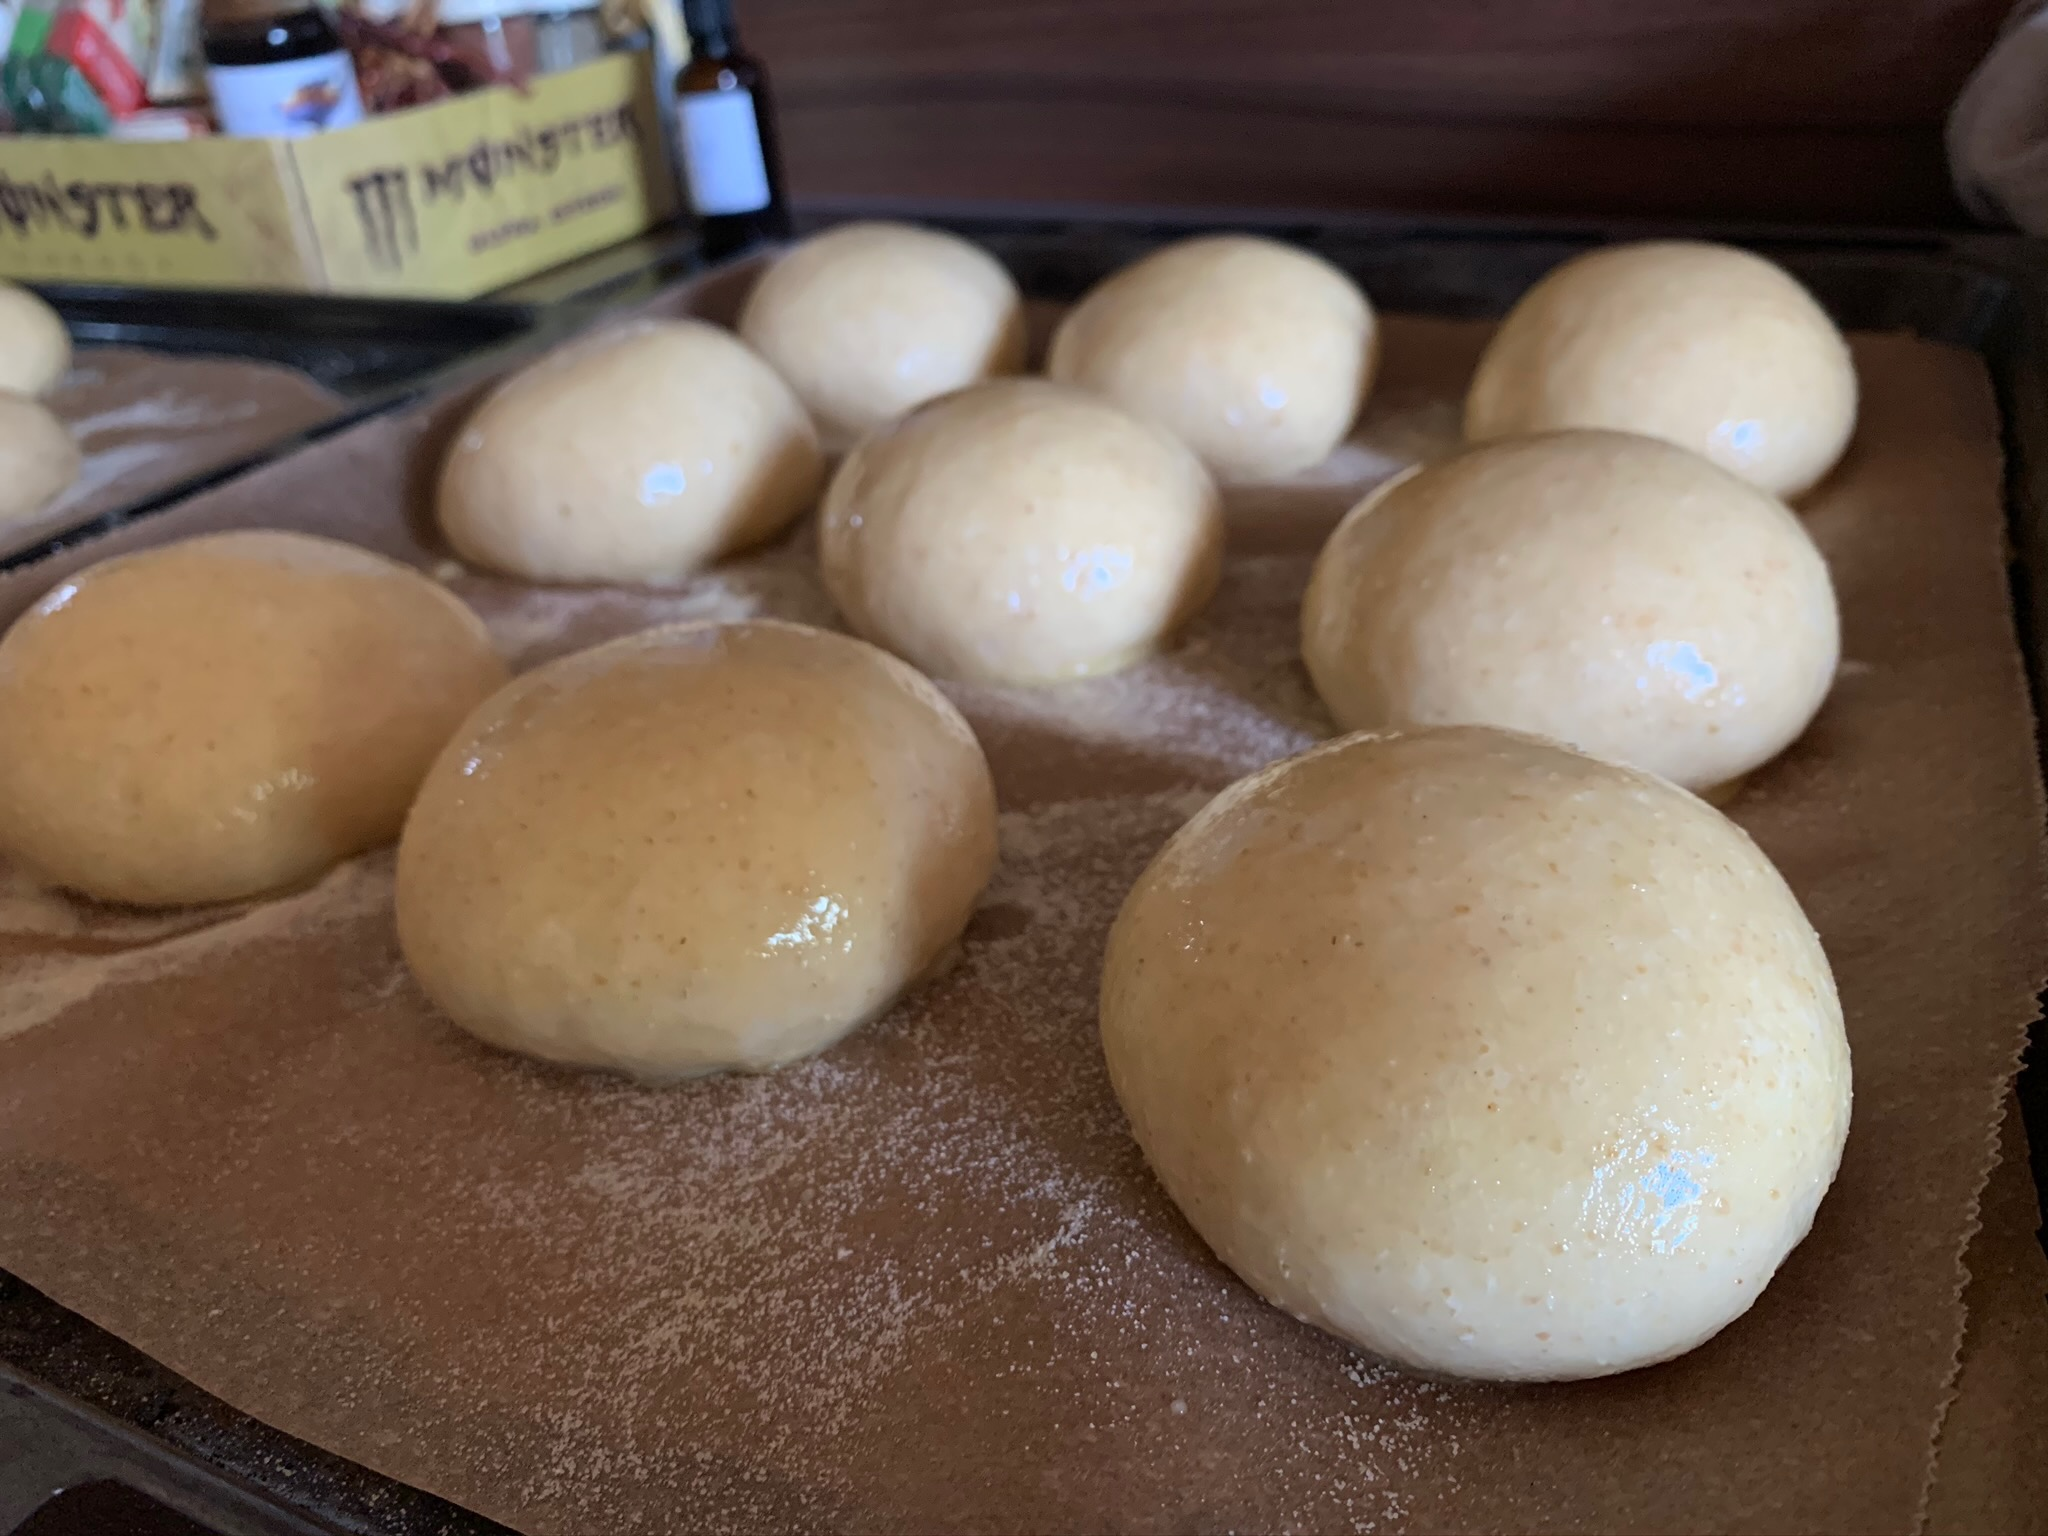
\includegraphics[width=\textwidth]{brioche-buns-before-baking}
    \caption{Brioche buns ready to be made. This time they have been made with
    an addition of 20\% whole-wheat.}
\end{figure}

\noindent\textbf{Instructions:}
\begin{center}
\begin{tabular}{|c|p{12cm}|}
    \hline
    \textbf{Step} & \textbf{Instruction} \\
    \hline
    1 & Mix everything together. Wait for 20~minutes and knead for 5~minutes.
    The dough should not be overly wet and sticky. If it is too sticky, proceed
    and add more flour. Knead a bit more and wait 20~minutes. Make a smooth
    dough ball so that the surface you are touching is not too sticky. \\
    \hline
    2 & Stretch and fold once after around 30 minutes. \\
    \hline
    3 & Wait until dough doubled in size, for sourdough aim for a 50\% size
    increase. Stretch and fold for sourdough whenever you see the dough
    flattens out a lot. \\
    \hline
    4 & Preshape into equally portioned dough balls. Make sure they are nice
    and smooth. Do not shape buns, the pre-shaping is sufficient. \\
    \hline
    5 & Place dough balls on a rack with parchment paper. Cover with a wetted
    kitchen towel so that they do not dry out. \\
    \hline
\end{tabular}
\end{center}

\noindent\textbf{Baking:}
To make the buns as soft as possible, make sure to bake them with as much steam
as possible. They are steamed all the way from the start to the end. If you
bake with too little steam they will turn dark too quickly and will be less
soft. Furthermore it is essential to bake at a lower temperature compared to
regular bread. This further improves softness. If you prefer a harder crust,
you can remove the source of steam once the buns no longer expand in size.

\begin{center}
\begin{tabular}{|c|p{12cm}|}
    \hline
    \textbf{Step} & \textbf{Instruction} \\
    1 & Once you see that they have increased by around 25\% in size preheat
    the oven to around 180°C (350°F). \\
    \hline
    2 & Cover buns with egg wash. To make the wash mix 1 egg with 100 ml of
    water. Place buns in the oven. Bake with as much steam as possible, this
    ensures that they become nice and soft. \\
    \hline
    3 & Bake until golden brown. This typically takes around 30 to 40 minutes. \\
    \hline
\end{tabular}
\end{center}

\begin{figure}[h]
    \centering
    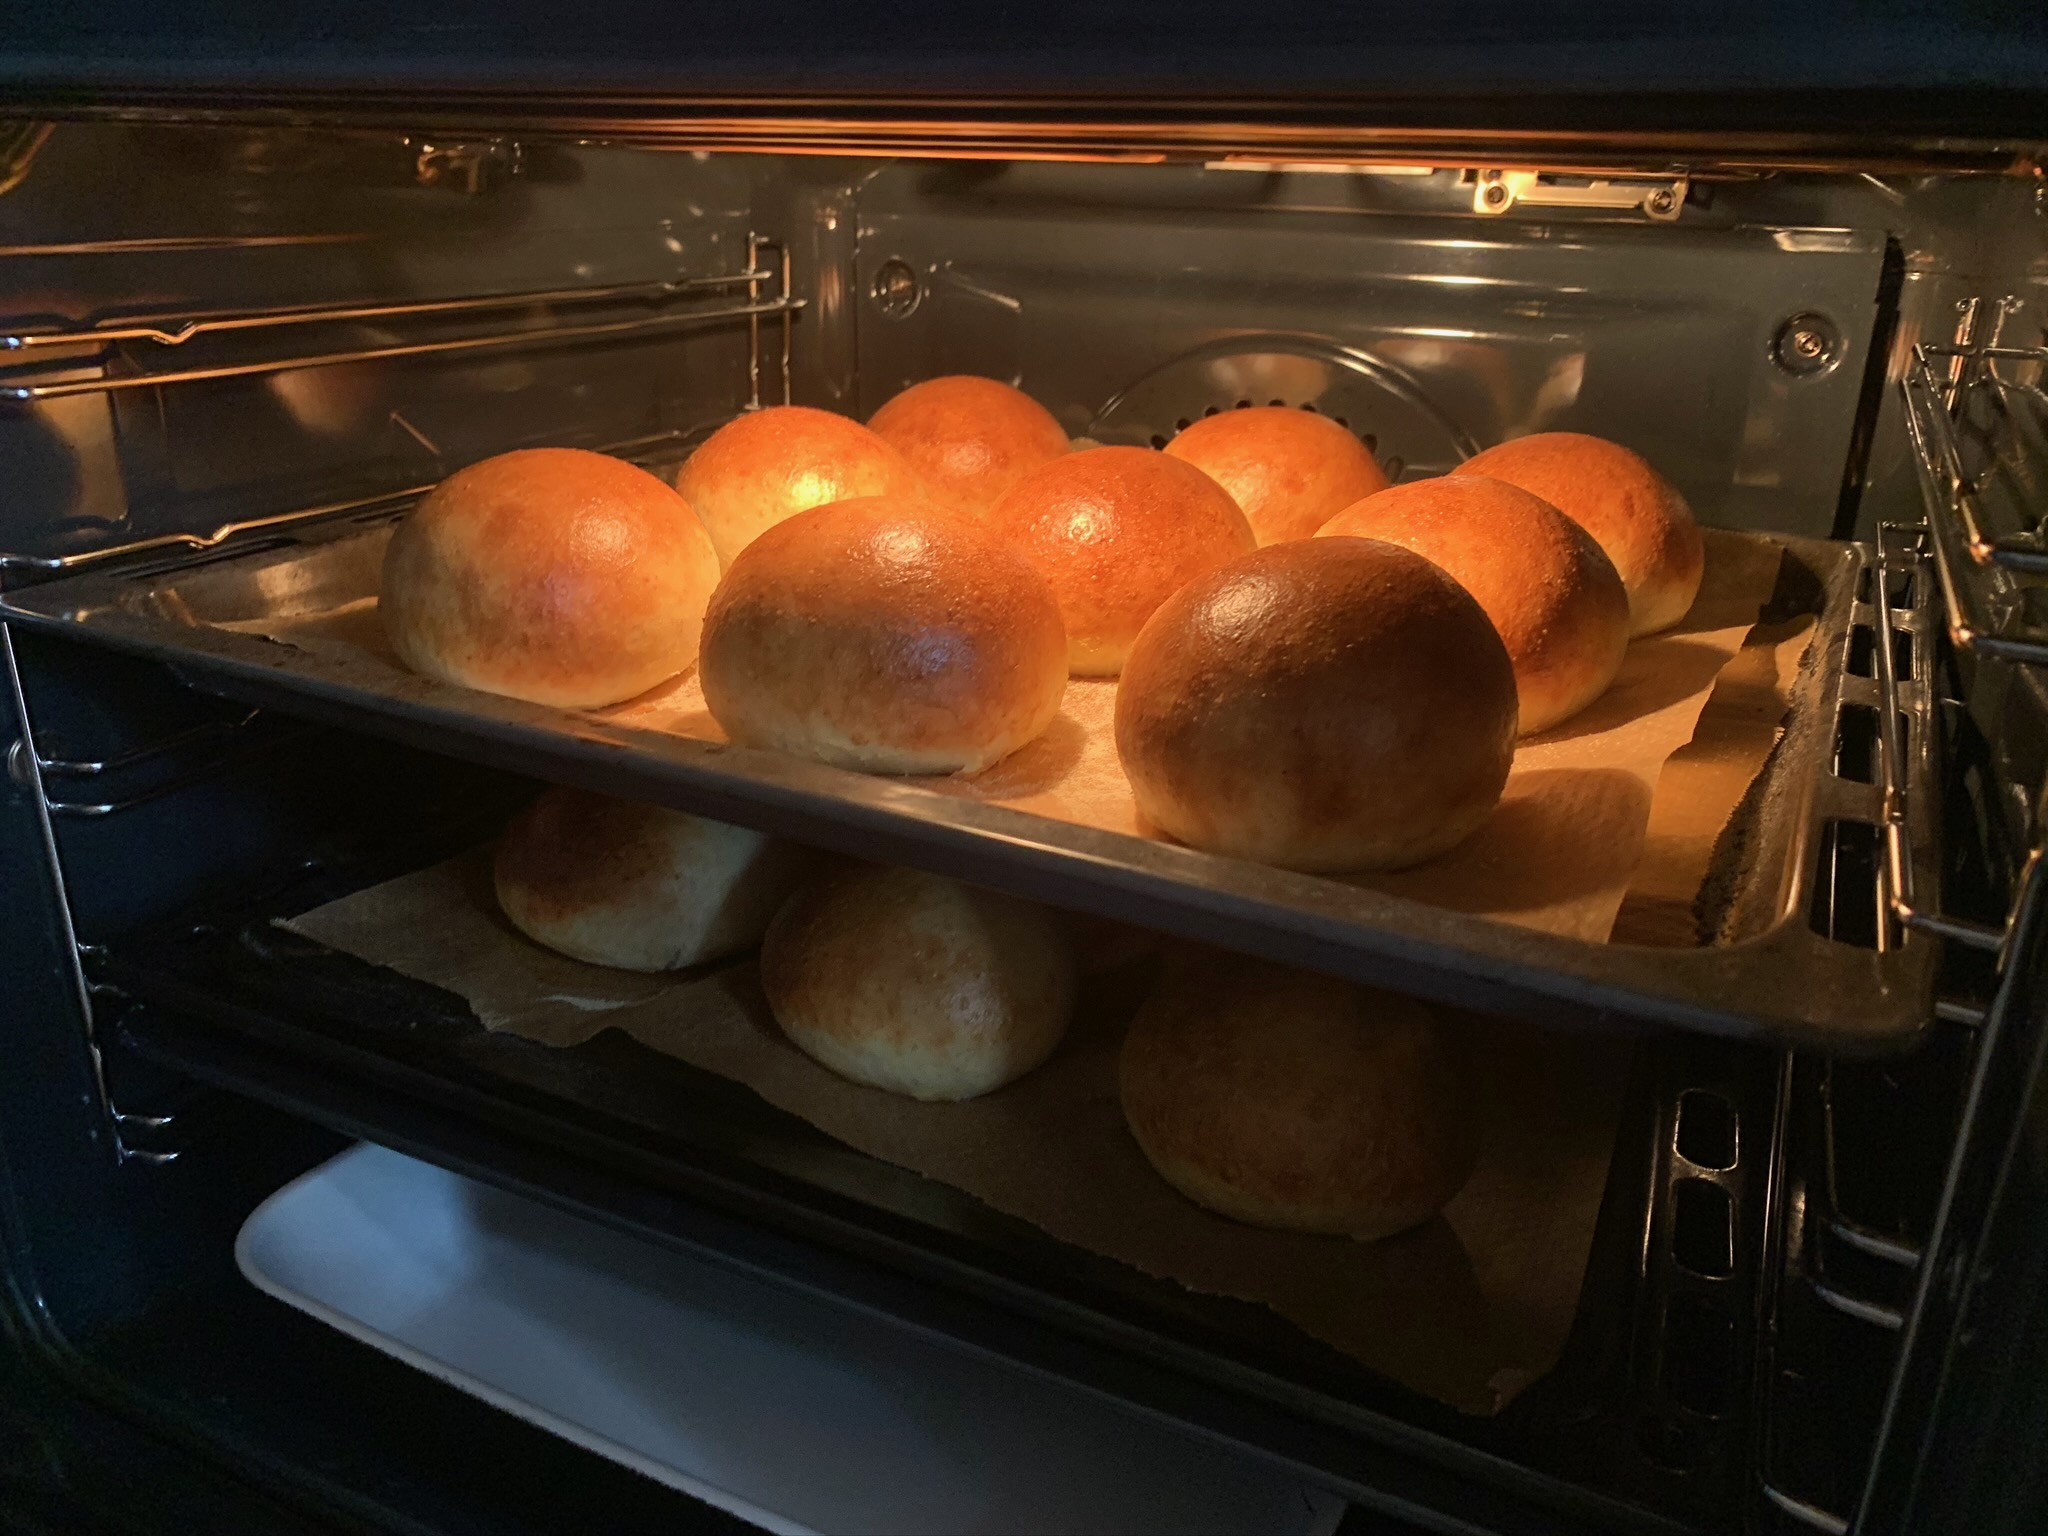
\includegraphics[width=\textwidth]{brioche-buns-baking}
    \caption{When baking more buns on 2~trays make sure to rotate the trays
    once while baking. This will ensure even browning and cooking times.}
\end{figure}
